We have presented in Section~\ref{sec:complexity-models} an abstract model made
to understand the asymptotic behaviour of our algorithms. In this chapter, we
present an alternative notion of complexity called \emph{bilinear complexity},
where the focus is on the number of multiplications needed to compute some map.
\minitoc

\begin{figure}[h]
  \centering
  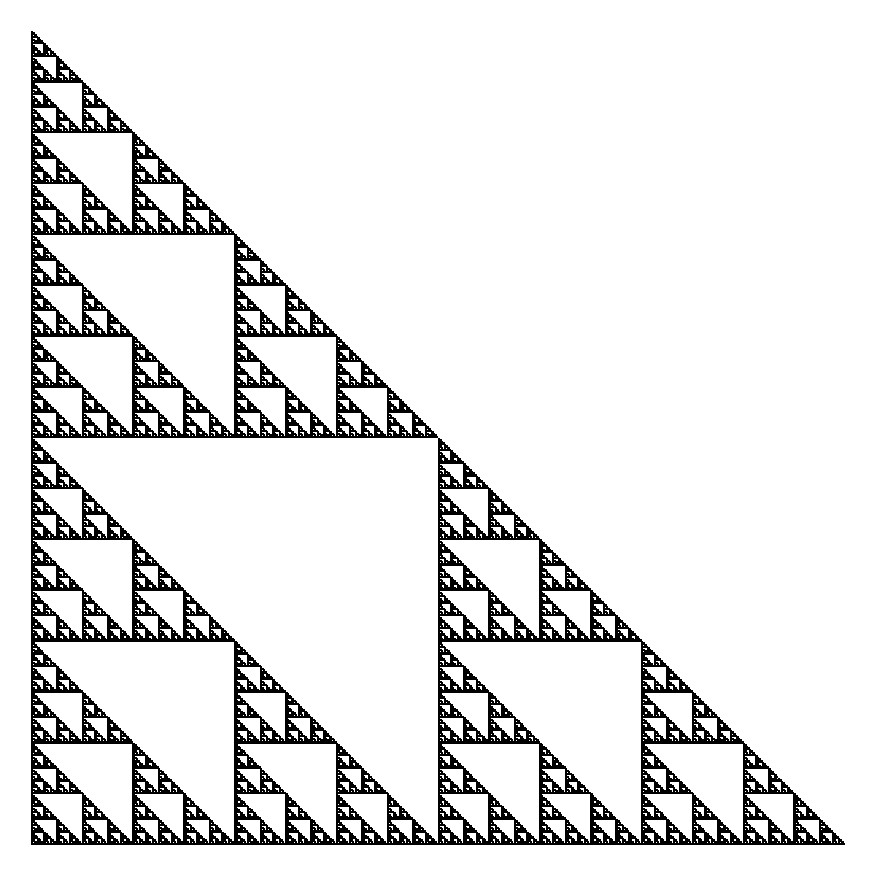
\includegraphics[scale=0.5]{img/karatsuba.pdf}
  \caption{Representation of Karatsuba's algorithm complexity.}
  \label{fig:karatsuba}
\end{figure}
\clearpage

\section{Bilinear complexity}

In the \emph{algebraic complexity model}~\cite{BCS13}, we assume that our
machine is able to perform any operation in some base field $\K$ in constant,
unit time. This is an idealized model made in order to simplify the
computation of the complexity of algebraic algorithms. Nevertheless,
multiplication of two variable quantities in $\K$ is arguably more expensive
than addition, or than multiplication of a variable by a fixed constant. In the
context of the computation of bilinear maps, extensive work has been done to
reduce the number of $2$-variable multiplications involved. Notable examples are
Karatsuba's algorithm~\cite{Karatsuba63} and
Strassen's algorithm~\cite{Strassen69}. Karatsuba's algorithm is
based on the fact that the bilinear map associated to the product of two
polynomials of degree $1$
\[
  A = a_1 X + a_0\text{ and }B = b_1 X + b_0
\]
can be computed with three products
\[
  c_0 = a_0b_0,
\]
\[
  c_1 = (a_0+a_1)(b_0+b_1),
\]
and
\[
  c_\infty = a_1b_1,
\]
instead
of the four classic ones $a_0b_0$, $a_0b_1$, $a_1b_0$ and $a_1b_1$ as follows:
\[
  AB = c_\infty X^2 + (c_1-c_\infty-c_0) X + c_0.
\]
It will become clear in Section~\ref{sec:evalinter} why we use the index
$\infty$ instead of $2$ for $c_\infty = a_1b_1$. Strassen's algorithm
exploits a similar idea in the case of $2\times2$ matrices: only $7$ products
are used instead of $8$ in order to compute a matrix product. Both these
algorithms have very practical consequences. Karatsuba's algorithm is used in
computer algebra softwares, when the standard multiplication is no longer
optimal, and when the Discrete Fourier Transform (DFT) is not yet the fastest.
Strassen's algorithm, used reccursively, is the fastest strategy available for
large matrix multiplication. Both these questions are treated in~\cite{GG13}.
Thus the idea of minimizing the number of multiplications, even if it means
having to compute more additions and substractions, seems a good idea.

The \emph{bilinear complexity}
$\mu(\Phi)$ of a bilinear map $\Phi$ over $\K$ represents the minimum number of two-variable
multiplications in a formula that computes $\Phi$, discarding the cost of other
operations such as addition or multiplication by a constant. In other words, in
this model of computation, we only count $2$-variable multiplications, and other
operations are assumed to have no cost. It is motivated by the fact that
$2$-variable multiplication is often more expensive to compute than other
operations and by the practicality of algorithms minimizing the multiplications,
such as Karatsuba's and Strassen's.
In particular when $\A$ is a finite dimensional algebra over $\K$,
we define the bilinear complexity of $\A$ as $\mu(\A/\K)=\mu(m_{\A})$
where $m_{\A}:\A\times\A\to\A$ is the multiplication map in $\A$ seen
as a $\K$-bilinear map.

Let $\K^{2\times2}$ be the algebra
of $2\times2$ matrices over $\K$. We know thanks to Strassen's algorithm that
\[
  \mu(\K^{2\times 2}/\K) \leq 7.
\]
In fact, this is optimal, so we have exactly $\mu(\K^{2\times2}/\K)=7$. In
general, it seems to be hard to find the bilinear complexity of a given algebra,
for example the bilinear complexity of $\K^{3\times3}$ is not known.
In the litterature, work has been done both to algorithmically find the bilinear complexity of
small algebras~\cite{BDEZ12, Covanov19} and to understand how the bilinear
complexity asymptotically grows~\cite{CC88, BCPRRR19}. Chudnovsky and Chudnovsky
proved in 1988 that the bilinear complexity of an extension field
$\mathbb{F}_{q^k}/\mathbb{F}_{q}$ is linear in the degree $k$ of the
extension, using an evaluation-interpolation method on curves. We present this
method in Section~\ref{sec:evalinter}.

\paragraph{Bilinear formulas.}

We can precisely define bilinear complexity with \emph{bilinear formulas}. We
also sometimes use the terms \emph{bilinear decomposition}, or \emph{bilinear
algorithm}, but it is really the same notion.
\begin{defi}[Bilinear formula]
  \label{defi:bilinear-formula}
  Let $V_1, V_2$ and $W$ be three finite dimensional vector spaces over $\K$ and 
  \[
    \Phi:V_1\times V_2\to W
  \]
  a bilinear map. A \emph{bilinear fomula}, or \emph{bilinear decomposition}, or
  \emph{bilinear algorithm} of length $n$ for $\Phi$ is a
  collection of $2n$ linear forms $\varphi_1, \dots, \varphi_n$ and $\psi_1,
  \dots, \psi_n$, and $n$ vectors $w_1, \dots, w_n$ in $W$ such that for all
  $x\in V_1$ and $y\in V_2$, we have
  \[
    \Phi(x, y) = \sum_{j=1}^n \varphi_j(x)\psi_j(y)w_j.
  \]
\end{defi}
Let $V_1$ and $V_2$ be $\K$-vector spaces of respective dimensions $l$ and $m$
and let
\[
  x = (x_1, \dots, x_l)\in V_1
\]
and
\[
  y = (y_1, \dots, y_m)\in V_2
\]
be two vectors.
A bilinear formula of length $n$ for a bilinear map $\Phi$ is essentially a way
of computing $\Phi(x, y)$ using a number $n$ of $2$-variable multiplicaitons in $\K$.
Indeed, for each $1\leq j \leq n$ we have
\[
  \varphi_j(x) = \sum_{i=1}^l a_{i, j}x_i
\]
and
\[
  \psi_j(y) = \sum_{i=1}^m b_{i, j}y_i
\]
where the elements $a_{i, j}$ and $b_{i, j}$ are \emph{constants} depending only
on $\Phi$. Thus the evaluation
\[
  \varphi_j(x)\psi_j(y)
\]
only requires one $2$-variable multiplication. The vectors $w_j\in W$ are also
constants depending only on $\Phi$, so we still need one $2$-variable
multiplication to compute 
\[
  \varphi_j(x)\psi_j(y)w_j.
\]
We said that the bilinear complexity measures the minimal number of
$2$-multiplication needed to compute a bilinear map $\Phi$. Knowing that a
bilinear formula of length $n$ for $\Phi$ implies that we can compute $\Phi$
with the same number $n$ of $2$-variable multiplication, the definition of
bilinear complexity follows.
\begin{defi}[Bilinear complexity]
  Let $V_1, V_2$ and $W$ be three finite dimensional vector spaces over $\K$ and 
  \[
    \Phi:V_1\times V_2\to W
  \]
  a bilinear map. The \emph{bilinear complexity} 
  \[
    \mu(\Phi)
  \]
  of $\Phi$ is the minimal length $n$ of a bilinear formula for $\Phi$.
\end{defi}
Equivalently, we can define the bilinear complexity as the rank of the tensor in 
\[
  V_1^\vee \times V_2^\vee \times W
\]
corresponding to $\Phi$, where $V_1^\vee$ (resp. $V_2^\vee$) is the dual space
of $V_1$ (resp. $V_2$).
\begin{ex}
  \label{ex:bilinear-complexity}
  Let $\K=\mathbb{F}_2$ and $V_1=V_2=W=(\mathbb{F}_2)^2$. We consider the
  bilinear map $\Phi$ that follows.
\[
\begin{array}{llcl}
  \Phi:&(\mathbb{F}_2)^2\times (\mathbb{F}_{2})^2&\to&(\mathbb{F}_2)^2\\
  &((x_0, x_1), (y_0, y_1))&\mapsto&(x_0y_0+x_1y_1, x_0y_1+x_1y_0+x_1y_1)
\end{array}
\]
Let $e_0=(1,0)$ and $e_1=(0,1)$ the vectors of the cannonical basis of
$(\mathbb{F}_{2})^2$, and let $e_0^\vee$ and $e_1^\vee$ the vectors of the dual
basis, \ie the linear forms $e_0^\vee$ and $e_1^\vee$ are given by
\[
\begin{array}{llcl}
  e_0^\vee:&(\mathbb{F}_2)^2&\to&\mathbb{F}_2\\
  &(x_0, x_1)&\mapsto&x_0
\end{array}
\]
and
\[
\begin{array}{llcl}
  e_1^\vee:&(\mathbb{F}_2)^2&\to&\mathbb{F}_2\\
  &(x_0, x_1)&\mapsto&x_1
\end{array}.
\]
Let $x = (x_0, x_1)$ and $y = (y_0, y_1)$, we have 
\begin{align*}
  \Phi(x,y) &= (x_0y_0+x_1y_1, x_0y_1+x_1y_0+x_1y_1) \\
  &= (x_0y_0, x_0y_0)+(x_1y_1, 0)+(0, (x_0+x_1)(y_0+y_1)) \\
  &=
  e_0^\vee(x)e_0^\vee(y)(e_0+e_1)+e_1^\vee(x)e_1^\vee(y)e_0+(e_0^\vee+e_1^\vee)(x)(e_0^\vee+e_1^\vee)(y)e_1.
\end{align*}
This last line is a bilinear formula of length $3$ for $\Phi$, and we can check
that no formula of length $2$ exists. Therefore the bilinear complexity of
$\Phi$ is 
\[
  \mu(\Phi) = 3.
\]
Equivalently, the tensor in
$((\mathbb{F}_2)^2)^\vee\otimes((\mathbb{F}_2)^2)^\vee\otimes(\mathbb{F}_2)^2$
corresponding to $\Phi$ is
\begin{align*}
  \widetilde{\Phi} &= e_0^\vee\otimes e_0^\vee\otimes e_0 + e_1^\vee\otimes
  e_1^\vee\otimes e_0 + e_0^\vee\otimes e_1^\vee\otimes e_1 + e_1^\vee\otimes
  e_0^\vee\otimes e_1 + e_1^\vee\otimes e_1^\vee\otimes e_1 \\
  &= e_0^\vee\otimes e_0^\vee\otimes(e_0+e_1)+e_1^\vee\otimes
  e_1^\vee\otimes e_0+(e_0^\vee+e_1^\vee)\otimes (e_0^\vee+e_1^\vee)\otimes e_1,
\end{align*}
and we can check that no smaller decomposition of $\widetilde\Phi$ into a sum of simple
tensors $a\otimes b\otimes c$ exist,
so we also see that the rank of the tensor $\widetilde\Phi$ is $3$.
\end{ex}
When the spaces $V_1$ and $V_2$ are equal
\[
  V_1 = V_2 = V
\]
the bilinear maps 
\[
  \Phi:V\times V\to W
\]
can be symmetric, \ie they can verify that, for all $x, y\in V$
\[
  \Phi(x, y) = \Phi(y, x).
\]
In that case, it is natural to investigate the existence and the length of
\emph{symmetric bilinear formulas}, \ie bilinear formulas where the linear forms
$\varphi_j$ and $\psi_j$ are equal, for all $j$. On an algorithmtic point of
view, it should also be easier to find all such formulas because the
search space is smaller. It is also easier to represent such formulas because we
only need to store $n$ linear forms instead of $2n$.
\begin{defi}[Symmetric bilinear formula]
  \label{def:sym-bil-for}
  Let $V$ and $W$ be two finite dimensional vector spaces over $\K$ and 
  \[
    \Phi:V\times V\to W
  \]
  a symmetric bilinear map. A \emph{symmetric bilinear fomula}, or
  \emph{symmetric bilinear decomposition}, or
  \emph{symmetric bilinear algorithm} of length $n$ for $\Phi$ is a
  collection of $n$ linear forms $\varphi_1, \dots, \varphi_n$
  and $n$ vectors $w_1, \dots, w_n$ in $W$ such that for all
  $x, y\in V$, we have
  \[
    \Phi(x, y) = \sum_{j=1}^n \varphi_j(x)\varphi_j(y)w_j.
  \]
\end{defi}
\begin{defi}[Symmetric bilinear complexity]
  \label{def:sym-bil-com}
  Let $V$ and $W$ be two finite dimensional vector spaces over $\K$ and 
  \[
    \Phi:V\times V\to W
  \]
  a bilinear map. The \emph{symmetric bilinear complexity} 
  \[
    \musym(\Phi)
  \]
  of $\Phi$ is the minimal length $n$ of a symmetric bilinear formula for
  $\Phi$.
\end{defi}
In other words, a symmetric bilinear formula is a bilinear formula where the
domain spaces are equal: $V_1=V_2$; and such that for all $1\leq j\leq n$,
the linear forms $\varphi_j=\psi_j$ are equal too. Note that it is not
clear from Definition~\ref{def:sym-bil-for} that a
\emph{symmetric} bilinear formula always
exists for symmetric bilinear maps, but it is indeed
true~\cite[Lemma $1.6$]{Randriam12}, thus
Definiton~\ref{def:sym-bil-com} makes sense. The formula obtained in
Example~\ref{ex:bilinear-complexity} is an example of bilinear formula that is
also a symmetric bilinear formula, therefore the symmetric bilinear complexity
is the same as the bilinear complexity in that case. We are particularly
interested in algebras $\A$ of the form
\[
  \A = \mathbb{F}_{q^k}[T]/(T^l)
\]
and for that reason we introduce a special notation for the bilinear complexity
of those algebra
\[
  \mu_q(k, l) = \mu(\A/\K).
\]
Among these algebras, the case $l=1$, where the algebra $\A$ is a finite field
extension of $\mathbb{F}_q$ of degree $k$ also plays a special role, so we
define 
\[
  \mu_q(k) = \mu_q(k, 1).
\]
Because these algebras are all commutative, the product 
\[
\begin{array}{lccl}
  m_\A:&\A\times \A&\to&\A\\
  &(x, y)&\mapsto&xy
\end{array}
\]
is a symmetric bilinear map, and we define the symmetric bilinear complexity of
the algebra $\A$ as the symmetric bilinear complexity of $m_\A$
\[
  \musym(\A) = \musym(m_\A).
\]
We also define the quantities
\[
  \musym_q(k, l)
\]
and 
\[
  \musym_q(k)
\]
the same way it was done for the usual bilinear complexity. Since a symmetric
bilinear formula is in particular a bilinear formula, we have for all $k\geq1$
and $l\geq1$
\[
  \mu_q(k, l)\leq\musym_q(k, l).
\]
In the other direction, we know (\cite[Theorem $1$]{SL84} or \cite[Lemma
$1.6$]{Randriam12}) that when the characteristic of $\A$ is not $2$,
or equivalently when $k$ is not a power of $2$ , that we have
\[
  \musym_q(k, l)\leq2\mu_q(k, l).
\]
Finally, we have no example of algebra $\A = \mathbb{F}_{q^k}[T]/(T^l)$ where the
quantities $\mu_q(k, l)$ and $\musym_q(k, l)$ are different when $q\geq3$.
% TODO: elaborate on this, is it true for q = 2?
% see for example
% [ 0 1 ]
% [ 1 0 ]
% ~~~~~~~~~~~~~~
% but that one does *not* come from a *regular* algebra A does it? If we take a
% counter example it has to have in the same realm as the fact that we are
% stating. 

\section{Chudnovsky-Chudnovsky algorithm}
Chudnovsky and Chudnovsky algorithm is based on evaluation-interpolation on
curves, we thus begin by presenting this principle.
\subsection{Evaluation - Interpolation}
\label{sec:evalinter}

Let $P\in\K[x]$ be a polynomial with coefficients in a finite field $\K$. The
evaluation-interpolation strategy is based on two facts:
\begin{itemize}
  \item a polynomial of degree $n$ can be described by its values at $n+1$
    points and reconstructed via \emph{interpolation};
  \item the \emph{evaluation} map at some point $a\in\K$ is a homomorphism of ring from
    $\K[x]$ to $\K$.
\end{itemize}
\paragraph{Interpolation.} The fact that a polynomial $P\in\K[x]$ of degree $n$
is uniquely determined by its values at $n+1$ (different) points in $\K$ follows
from the fact that a polynomial of degree $n$ with coefficients in $\K$ has up
to $n$ roots. This gives us the \emph{uniqueness} of the polynomial. As for the
\emph{existence}, it follows from the Lagrange interpolation. Let $x_1, \dots,
x_{n+1}\in\K$ be $n+1$ points in $\K$ and $y_1, \dots, y_{n+1}$ the
corresponding evaluation values, such that
\[
  \forall j\in\left\{ 1, \dots, n+1 \right\},\,y_j = P(x_j).
\]
Let 
\[
  L_j = \prod_{i\neq j}\frac{x-x_i}{x_j-x_i},
\]
we then have $L_j(x_i) = \delta_{i, j}$ with
\[
  \delta_{i, j} = 
  \left\{\begin{array}{ll}
      1&\mbox{if } i=j\\
      0&\mbox{if } i\neq j
    \end{array}
    \right.
\]
the Kronecker symbol. Now, the polynomial
\[
  P = \sum_{j=1}^{n+1} y_j L_j
\]
meets all the evaluation conditions and is the sum of polynomials of degree $n$
so $P$ is of degree at most $n$.

\paragraph{Evaluation.} Let $P, Q\in\K[x]$ be two polynomials with coefficients
in $\K$ and $a\in\K$, then we have
\[
  (P+_{\K[x]}Q)(a) = P(a) +_{\K} Q(a)
\]
and 
\[
  (P\times_{\K[x]} Q)(a) = P(a) \times_{\K} Q(a),
\]
where $+_{\K[x]}, \times_{\K[x]}$ (resp. $+_{\K}, \times_{\K})$ are the addition
and multiplication operations in $\K[x]$ (resp. $\K$).
In other words, the map
\[
\begin{array}{lccl}
  \textrm{ev}_a:&\K[x]&\to&\K\\
  &P&\mapsto&P(a)
\end{array}
\]
is an homomorphism of rings from $\K[x]$ to $\K$.

We are used to represent polynomials by their coefficients, but these two facts
suggest that we can also represent polynomials by their values at some points.
With this representation, adding two polynomials is done by adding the
values, which is done with linear complexity, the same as with the coefficient
representation. But the multiplication of polynomials is also obtained via the
multiplication of the values, which is linear again and better than the
quadratic complexity obtained with the usual multiplication formula for the
coefficients. An important problem is then to be able to change between
representations at a small cost, this is done using well-chosen points of
evaluation and this strategy is known under the name of Fast Fourier
Transform (FFT)~\cite{GG13}. Let $P, Q\in\K[x]$ be two polynomials with
coefficients in $\K$ represented by their coefficients, such that
$\deg(PQ)=n-1$. In order to multiply $P$ and $Q$ we need at least $n$ points in
$\K$ and the evaluation-interpolation strategy consists in $3$ steps:
\begin{enumerate}
  \item multipoint evaluation of $P$ and $Q$ at $n$ points $a_1, \dots, a_n$;
  \item coordinate-wise multiplication;
  \item interpolation to reconstruct the product $PQ$.
\end{enumerate}
When there are not enough points in $\K$ to use this method, instead of
evaluating on points of $\K$, we can evaluate the polynomials on points of
curves on $\K$ with enough points. As a first example, we can interpret
Karatsuba's algorithm as an evaluation-interpolation scheme on
the projective line $\mathbb{P}^1(\K)$. Let 
\[
  P = a_1 x + a_0
\]
and 
\[
  Q = b_1 x + b_0,
\]
then
\[
  c_0 = \textrm{ev}_0(P)\textrm{ev}_0(Q) = a_0b_0
\]
is obtained via evaluation at $0$,
\[
  c_1 = \textrm{ev}_1(P)\textrm{ev}_1(Q) = (a_0+a_1)(b_0+b_1)
\]
is obtained via evaluation at $1$, and
\[
  c_\infty = \textrm{ev}_\infty(P)\textrm{ev}_\infty(Q) = a_1b_1
\]
is obtained via evaluation at the point at infinity, where the evaluation at
infinity $\textrm{ev}_{\infty}$ is the function mapping a polynomial to its
leading coefficient. This strategy can be generalized to curves (or their
function fields) more complex
than $\mathbb{P}^1(\K)$, as was done by Chudnovsky and Chudnovsky in
$1988$~\cite{CC88}.

\subsection{Asymptotic complexity}

In 1988, Chudnovsky and Chudnovsky~\cite{CC88} extended the idea of polynomial
interpolation to interpolation on rational places, \ie places of degree $1$, of
a function field. It led to an algorithm for the finite field product with an
asymptotically linear complexity in the extension degree. We first present the historical theorem
in~\cite{CC88}.
\begin{thm}
  \label{thm:CC88}
  Let $F$ be a function field over $\mathbb{F}_q$.
  Assume there exist a place $Q\in\mathbb{P}_{F}$ of $F$ of degree $k$, $P_1,
  \dots, P_n\in\mathbb{P}_F$ places of $F$ of degree $1$, and a divisor
  $D\in\D_F$ of $F$ such that the places $Q$ and $P_1, \dots, P_n$ are not in
  the support of $D$ and such that the following conditions hold.
  \begin{enumerate}[(i)]
    \item \label{cond:1} The evaluation map
      \[
        \begin{array}{cccc}
        \ev_{Q, D}: & L(D) & \to & \mathbb{F}_{q^k}\\
  & f & \mapsto & f(Q)
\end{array}
\]
is \emph{surjective}.
    \item \label{cond:2} The evaluation map
      \[
        \begin{array}{cccc}
        \ev_{\Pcal, 2D}: & L(2D) & \to & (\mathbb{F}_{q})^n\\
  & h & \mapsto & (h(P_1), \dots, h(P_n))
\end{array}
\]
is \emph{injective}.
  \end{enumerate}
  Then the product in the extension field 
  \[
    \mathbb{F}_{q^k}/\mathbb{F}_q
  \]
  admits a symmetric formula of length $n$, \ie we have $\musym_q(k)\leq n$.
\end{thm}

\section{Algorithmic searches in small dimension}

% Contents
% ========
%
% - Barbulescu, Detrey, et al 
% - Covanov 

The last results based on Chudnovsky and Chudnovsky algorithm allow us to find
one decomposition, and thus give us an (asymptotic) upper bound on the bilinear
complexity of algebras
\[
  \A = \mathbb{F}_{q^k}[T]/(T^l).
\]
When one wants to find the exact value of the bilinear complexity of a given
bilinear map $\Phi$, one can either find all bilinear formulas for $\Phi$, or
find a theoretical argument to directly find the bilinear complexity of $\Phi$. The latter
solution is often hard, and there also exist some in-between approaches such
as finding a bilinear formula of a given length and proving that no shorter formula
could exist. Still, because it seems hard to directly find the bilinear
complexity of a bilinear map, algorithms were developped to find bilinear
formulas. These algorithms are essentially exhaustive searches, so they 
have an exponential complexity, but they also exploit the eventual symmetries
in the definition of $\Phi$ to eliminate a lot of potential candidates along the
way, in order to be as efficient as possible in practice. We first see
Barbulescu, Detrey, Estibals and Zimmerman's algorithm~\cite{BDEZ12}.

\subsection{Barbulescu, Detrey, Estibals and Zimmerman's algorithm}

In $2012$, Barbulescu, Detrey, Estibals and Zimmerman published a new framework
to find bilinear formulas for arbitrary bilinear maps over finite fields. Let
$V_1$, $V_2$ and $W$ be three finite dimensional $\K$-vector space of respective
dimension $l$, $m$, and $n$, such that we have
\[
  V_1\cong\K^l\hspace{3cm}V_2\cong\K^m\hspace{3cm}W\cong\K^n.
\]
Let
\[
  \Phi:V_1\times V_2\to W
\]
be a bilinear map, and denote by $\B$ the space of bilinear \emph{forms} from
$V_1\times V_2$ to $\K$. Let $\gamma\in\B$ a bilinear form, then if
\[
  x = (x_1, \dots, x_l)\in V_1
\]
and
\[
  y = (y_1, \dots, y_m)\in V_2,
\]
then $\gamma$ is given by
\[
  \gamma(x, y) = \sum_{i=1}^{l}\sum_{j=1}^m \gamma_{i, j} x_i y_j.
\]
Hence, $\B$ is a $\K$-vector space of dimension $lm$ and we can see $\gamma$ as
a vector
\[
  \gamma = (\gamma_{1, 1}, \dots, \gamma_{l, m}).
\]
An other interesting representation is to see $\gamma$ as a $l\times m$ matrix
\[
  G = (\gamma_{i, j})_{i, j},
\]
such that $\gamma$ is given by
\[
  \gamma(x, y) = x G y^t
\]
where $y^t$ is the transposed of $y$ and thus $y^t$ is a column vector. We let
$\gamma_j$ be the $j$-th coordinate of $\Phi$ in $W$, such that
\[
  \Phi = (\gamma_1, \dots, \gamma_n).
\]
If $n=1$, $\Phi$ is a bilinear form and its bilinear complexity is given by the
rank of its matrix representation. The reason is that a rank $r$ matrix is the sum of $r$ matrices of rank $1$,
and a rank $1$ matrix corresponds to a bilinear form that can be evaluated using
only one $2$-variable multiplication. Indeed, let $A$ be a $l\times m$ matrix of rank $1$, we know that
there exist a nonzero vector 
\[
  b=(b_1, \dots, b_m)\in\K^m
\]
such that the rows $(r_j)_{1\leq j \leq m}$ of $A$, seen as vectors $\K^m$, are
all multiple of $b$, \ie for all $1\leq j \leq l$, we have
\[
  r_j = a_j b
\]
with $a_j\in\K$, and so
\[
  A =
\begin{bmatrix}
  & & & & a_1 b & & & & \\
  & & & & \vdots & & & & \\
  & & & & a_l b & & & & \\
\end{bmatrix}.
\]
Let $\gamma$ be the bilinear form represented by $A$, $x\in\K^l$ and $y\in\K^m$, then
\begin{align*}
  \gamma(x, y) &= x A y^t \\
  &= \sum_{i=1}^{l}(x_i \sum_{j=1}^m a_i b_j y_j) \\
  &= (\sum_{i=1}^l a_i x_i)\times(\sum_{j=1}^m b_j y_j).
\end{align*}
The elements $a_1, \dots, a_l$ and $b_1, \dots, b_m$ only depend on $\gamma$ (or
equivalently, on $A$), so they are constants, thus evaluating $\gamma$ only
requires one $2$-variable multiplication.
% TODO: give an example
When $n>1$, \ie $\Phi$ is not a
bilinear form, there is no similar way of knowing the bilinear complexity of
\[
  \Phi = (\gamma_1, \dots, \gamma_n).
\]
Nonetheless, Barbulescu \etal presented an algorithm to find bilinear formulas
for $\Phi$. The representation that is used for this algorithm is the vector
one, and the subspace
\[
  V = \Span\left\{ \gamma_1, \dots, \gamma_n \right\}\subset\B
\]
plays a central role. The general idea is to find a generating family of $V$ composed of
rank $1$ bilinear forms.
\begin{prop}
  Let $V_1$, $V_2$, and $W$ three finite $\K$-vector spaces and $\Phi:V_1\times
  V_2\to W$ a bilinear map such that
  \[
    \Phi = (\gamma_1, \dots, \gamma_n).
  \]
  Let 
  \[
    V = \Span\left\{ \gamma_1, \dots, \gamma_n \right\}
  \]
  and let 
  \[
    \mathcal F = \left\{ \phi_1, \dots, \phi_t \right\}
  \]
  be a generating family of $V$ composed of rank $1$ bilinear forms. Then there
  exists a bilinear formula of length $t$ for $\Phi$.
\end{prop}
\begin{proof}
 Let 
 \[
   \left\{ e_1, \dots, e_n \right\}
 \]
 be a basis of $W$.  For each $1\leq j \leq n$, let
 \[
   \gamma_j = \sum_{i=1}^t a_{i, j} \phi_i
 \]
 be a decomposition of $\gamma_j$ in the generating family $\mathcal F$.
 It follows that
 \begin{align*}
   \Phi &= \sum_{j=1}^n\gamma_j e_j \\
   &= \sum_{j=1}^n (\sum_{i=1}^ta_{i, j}\phi_i)e_j\\
   &= \sum_{i=1}^t \phi_i (\sum_{j=1}^n a_{i, j}e_j)\\
   &= \sum_{i=1}^t \phi_i w_i\\
 \end{align*}
 with, for all $1\leq i\leq t$,
\[
  w_i = \sum_{j=1}^n a_{i, j}e_j
\]
a (constant) vector in $W$ and $\phi_i$ is a rank $1$ bilinear form, so that
it can be evaluated using only one $2$-variable multiplication in $\K$. Therefore
we have a bilinear formula of length $t$ for $\Phi$.
\end{proof}
If $\Phi$ is a symmetric bilinear map, the same strategy can be used with a
basis composed of symmetric bilinear forms of rank $1$. Now the question is how
to find such generating family $\mathcal F$. Let 
\[
  \G = \left\{ \phi\in\B\,|\,\phi\text{ is of rank }1 \right\}
\]
be the set of bilinear forms of rank $1$. In order to find bilinear formulas of
length $t$, a naive solution is to exhaustively search for elements 
\[
  g_1, \dots, g_t\in\G
\]
such that
\begin{equation}
  V\subseteq\Span\left\{ g_1, \dots, g_t \right\}.
  \label{eq:subspace-cond}
\end{equation}
There is 
\[
  {\Card\G}\choose{t}
\]
possible choices for the $t$-uple $(g_1, \dots, g_t)$, and for each $t$-uple we
have to test the subspace condition~\eqref{eq:subspace-cond}. For the sake of
simplicity, we consider the \emph{combinatorial complexity} of this problem, \ie
we consider that all matrix operations have constant complexity (\eg computing
the dimension of a vector space, checking if a vector is in a vector space).
Thus the combinatorial complexity of this strategy is ${\Card\G}\choose{t}$.
Unfortunately, two different $t$-uple of generators in $\G$ can span the same
vector space, and so the naive algorithm is non optimal. Barbulescu \etal attack
this problem by looking directly at subspaces $W$ such that
\[
V\subseteq W.
\]
More precisely, if we want to find a length $t$ formula, we search at spaces $W$ such that
\begin{enumerate}[(i)]
  \item \label{enum:subspace} $V\subseteq W$;
  \item \label{enum:rank1} $\Span(W\cap\G) = W$, \ie $W$ is generated by rank $1$ bilinear forms;
  \item $\dim W = t$, \ie $k$ generators of $\G$ are needed.
\end{enumerate}
We remark thanks to~\ref{enum:subspace} that $V$ is contained in each space $W$
that we are looking for. Thus, we can search for spaces $W$ by adding elements
to $V$. Of course, there a lot of spaces verifying~\ref{enum:subspace}
alone, but this condition, together with~\ref{enum:rank1}, is in fact equivalent
to
\begin{enumerate}
  \item[(ii')] \label{enum:sum} $\exists\,\W\subset\G$ such that
    $W=V\oplus\Span\W$,
\end{enumerate}
therefore, we need only to add elements from $\G$ to $V$.
\begin{lm}
  \label{lm:cond-equiv}
  All spaces $W$ that verify~\ref{enum:subspace} and~\ref{enum:rank1} also
  verify~(ii').
\end{lm}
\begin{proof}
  Assume that conditions~\ref{enum:subspace} and~\ref{enum:rank1} are satisfied,
  let
  \[
    l = \dim V
  \]
  and
  \[
    m = \dim W.
  \]
  Let $B$ a basis of $W$ composed of elements of $G$, \ie rank $1$ bilinear
  forms. We construct a family $(\W_j)_{0\leq j\leq m-l}$ of subsets
  $\W_j\subset\G$ such that for all
  $0\leq j\leq m-l$
  \[
    \dim(V\oplus\Span\W_j) = l+j
  \]
  and
  \[
    V\oplus\Span\W_j \subseteq W.
  \]
  We let $\W_0=\emptyset$ be the nullspace, and we inductively construct $\W_j$
  for $1\leq j\leq m-l$. Assume that  $\dim(V\oplus\Span\W_{j-1}) = l+j-1$ and
  $V\oplus\Span\W_{j-1} \subseteq W$. We choose an element $\varphi$ in $B$ such
  that
  \[
    \varphi\notin V\oplus\Span\W_{j-1}.
  \]
  Such an element exists, otherwise we would have
  \[
    V\oplus\Span\W_{j-1}=W
  \]
  and so 
  \[
    \dim(V\oplus\Span\W_{j-1}) = l+j-1=\dim W = m.
  \]
  Since $j\leq m-l$, it would follow that
  \[
    m = l+j-1\leq m-1,
  \]
  a contradiction. Hence, we define 
  \[
    \W_j = \W_{j-1}\cup\left\{ \varphi \right\},
  \]
  and we have
  \[
    \dim(V\oplus\Span\W_j) = l+j
  \]
  and
  \[
    V\oplus\Span\W_j \subseteq W.
  \]
  We take the set $\W = \W_{m-l}$ and we have the desired property.
\end{proof}
Lemma~\ref{lm:cond-equiv} essentially tell us that the combinatorial complexity
of finding a length $t$ formula is
\[
  {\Card\G}\choose{t - \dim V}
\]
because we can take advantage of the fact that we already know that a solution
space $W$ verifies $V\subseteq W$. We introduce some more notation: we let
\[
  \mathcal S_t=\left\{ W\subseteq\B\,|\,\Span(W\cap\G)=W\text{ and } \dim W = t\right\}
\]
be the set of vector subspaces of $\B$ of dimension $t$ that are generated by
rank $1$ bilinear forms. We also let
\[
  \mathcal S_t(V)=\left\{ W\in\mathcal S_t\,|\,V\subseteq W \right\}
\]
the subspaces in $\mathcal S_t$ that also contain $V$. With this new
terminology, if we want to compute formulas of length $t$ for
\[
  \Phi = (\gamma_1, \dots, \gamma_n),
\]
our goal is now to compute $\mathcal S_t(V)$ with
\[
  V = \Span(\left\{ \gamma_1, \dots, \gamma_n \right\}.
\]
In order to effectively compute these sets, we use Algorithm~\ref{algo:rank1} to
check if a vector space is generated by rank $1$ bilinear forms.
\begin{algorithm}
  \caption{\textsc{HasRankOneBasis}}
  \label{algo:rank1}
  \begin{algorithmic}[1]
    \Require{$V\subseteq\B$ a subspace of $\B$ of dimension $l$}
    \Ensure{A boolean indicating if $V\in\mathcal S_l$}
    \State $\mathcal H\gets \Span(V\cap\G)$
    \If{$\dim\mathcal H=\dim V$}
    \State \Return{\True}
    \Else
    \State \Return{\False}
    \EndIf
  \end{algorithmic}
\end{algorithm}
The algorithm following Lemma~\ref{lm:cond-equiv} is described in
Algorithm~\ref{algo:BDEZ}.
\begin{algorithm}
  \caption{Barbulescu, Detrey, Estibals, Zimmerman}
  \label{algo:BDEZ}
  \begin{algorithmic}[1]
    \Require{$V\subseteq\B$ a subspace of $\B$.;
      $t\in\mathbb{N}$ an integer}
    \Ensure{A list of formulas of length $t$ for $\Phi$.}

    \Function{ExpandSubspace}{$X$, $\mathcal H$, $d$, $t$}
    \If{$d=t$ and $\dim X = t$ and \Call{HasRankOneBasis}{X}}
    \State \Return{$\left\{ X \right\}$}
    \Else
    \State $\mathcal S\gets\emptyset$
    \For{$i=1$ to $\Card \mathcal H$}\Comment{$\mathcal
      H=\left\{ \phi_1, \dots, \phi_v\right\}$}
      \State\label{line:SmodPhi} $\mathcal S\gets \left\{ \phi_{i+1}, \dots, \phi_v
  \right\}\mod\phi_i$\Comment{Gaussian elimination modulo $\phi_i$}
    \State $\mathcal S'\gets\mathcal
    S\cup\Call{ExpandSubspace}{X\oplus\Span(\phi_i), \mathcal H', d+1, t}$
    \EndFor
    \State \Return{$\mathcal S$}
    \EndIf
    \EndFunction
    \State $V=\Span(\left\{ \gamma_1, \dots, \gamma_n \right\})$
    \State\label{line:GmodV} \Return{\Call{ExpandSubspace}{$V$, $\G\mod V$, $\dim V$,
    $t$}}\Comment{Gaussian reduction of $\G$ modulo a basis of $V$}
  \end{algorithmic}
\end{algorithm}
There is an other advantage of Algorithm~\ref{algo:BDEZ} compared to the naive
algorithm. We see Line~\ref{line:SmodPhi} and Line~\ref{line:GmodV} that it
takes into account the equivalence relation ``modulo $V$'', \ie if there are two
elements $\phi$ and $\phi'$ of $\G$ such that 
\[
  V\oplus\Span\phi=V\oplus\Span\phi',
\]
only one representative is explored in the tree of recursive calls. As an
example, if
\[
  \G = \left\{ \phi_1, \phi_2, \phi_3, \phi_4 \right\}
\]
contains $4$ rank $1$ bilinear forms, and if $t - \dim V = 3$, the tree of
recursive calls would generically (\eg if the bilinear forms $\phi_j$ are
independent modulo $V$) look like Figure~\ref{fig:rec-call-tree}, where we let
\[
  W_{i} = \Span(\left\{ \phi_i\right\}),
\]
\[
  W_{i, j} = \Span(\left\{ \phi_i, \phi_j\right\}),
\]
and
\[
  W_{i, j, k} = \Span(\left\{ \phi_i, \phi_j, \phi_k \right\}).
\]
\begin{figure}
  \centering
  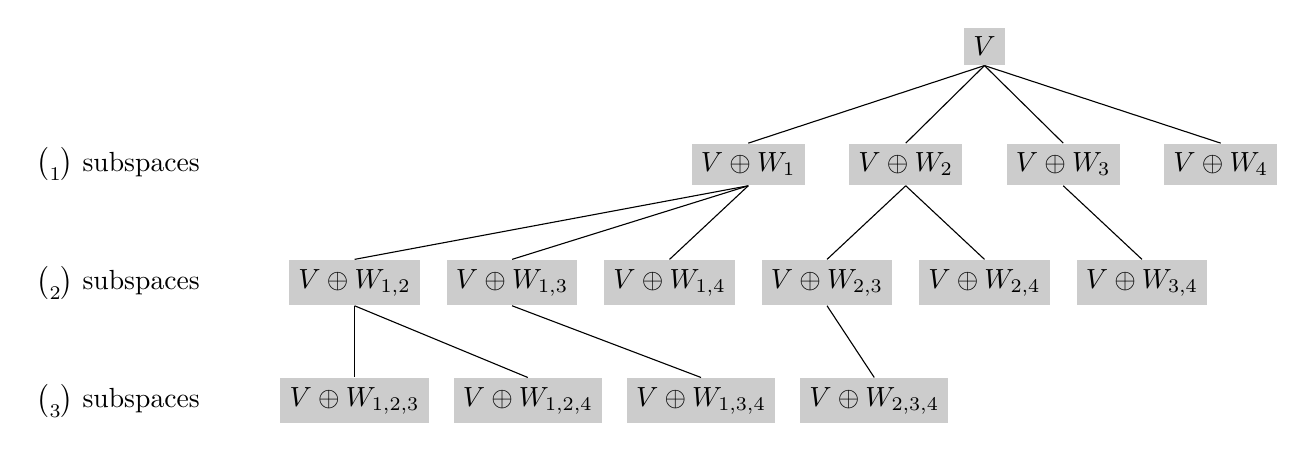
\begin{tikzpicture}
    \node[fill=black!20] (V) at (0,4.5) {$V$};
    \node[fill=black!20] (1) at (-3,3) {$V\oplus W_1$};
    \node[fill=black!20] (2) at (-1,3) {$V\oplus W_2$};
    \node[fill=black!20] (3) at (1,3) {$V\oplus W_3$};
    \node[fill=black!20] (4) at (3,3) {$V\oplus W_4$};

    \node[fill=black!20] (12) at (-8,1.5) {$V\oplus W_{1,2}$};
    \node[fill=black!20] (13) at (-6,1.5) {$V\oplus W_{1,3}$};
    \node[fill=black!20] (14) at (-4,1.5) {$V\oplus W_{1,4}$};

    \node[fill=black!20] (23) at (-2,1.5) {$V\oplus W_{2,3}$};
    \node[fill=black!20] (24) at (0,1.5) {$V\oplus W_{2,4}$};

    \node[fill=black!20] (34) at (2,1.5) {$V\oplus W_{3,4}$};

    \node[fill=black!20] (123) at (-8,0) {$V\oplus W_{1,2,3}$};
    \node[fill=black!20] (124) at (-5.8,0) {$V\oplus W_{1,2,4}$};
    \node[fill=black!20] (134) at (-3.6,0) {$V\oplus W_{1,3,4}$};
    \node[fill=black!20] (234) at (-1.4,0) {$V\oplus W_{2,3,4}$};

    \node (C1) at (-11, 3) {${\Card\G}\choose{1}$ subspaces};
    \node (C2) at (-11, 1.5) {${\Card\G}\choose{2}$ subspaces};
    \node (C3) at (-11, 0) {${\Card\G}\choose{3}$ subspaces};

    \draw (V.south) -- (1.north);
    \draw (V.south) -- (2.north);
    \draw (V.south) -- (3.north);
    \draw (V.south) -- (4.north);

    \draw (1.south) -- (12.north);
    \draw (1.south) -- (13.north);
    \draw (1.south) -- (14.north);
    \draw (2.south) -- (23.north);
    \draw (2.south) -- (24.north);
    \draw (3.south) -- (34.north);

    \draw (12.south) -- (123.north);
    \draw (12.south) -- (124.north);
    \draw (13.south) -- (134.north);
    \draw (23.south) -- (234.north);
  \end{tikzpicture}
  \caption{Tree of recursive calls in Algorithm~\ref{algo:BDEZ}, with
$\Card\G=4$ and $t-\dim V=3$.}
  \label{fig:rec-call-tree}
\end{figure}
Algorithm~\ref{algo:BDEZ} can also be adapted to to find \emph{symmetric}
formulas: instead of searching in the set $\G$, we search in the set
\[
  \G_\text{sym} = \left\{ \phi\in\B\,|\,\phi\text{ is symmetric and is of rank
  }1 \right\}.
\]
Since
\[
  \Card\G_\text{sym} = \sqrt{\Card\G},
\]
the complexity of Algorithm~\ref{algo:BDEZ} adapted to the symmetric case is
naturally better.
Although not initially published in~\cite{BDEZ12}, Barbulescu, Detrey, Estibals
and Zimmerman improved on their algorithms by using symmetries in the definition
of the subspaces of $\B$. Their strategy
was described in~\cite{Covanov19}, as well as further improvements from Covanov,
exploiting even more symmetries.
% TODO: add BDEZStab (i.e. the version with RP-automorphisms)? Is that
% necessary since we do not quite use that in the case of trisymmetric bilinear
% forms? Sould we also present Covanov's method?
% 
